\documentclass[twoside,leqno,twocolumn]{article}

% Comment out the line below if using A4 paper size
%\usepackage[letterpaper]{geometry}

\usepackage{ltexpprt}
\usepackage{hyperref}

% *** MATH PACKAGES ***
%
\usepackage{amsmath}
\usepackage{nicefrac}
\usepackage{array}
\usepackage{lmodern,amssymb}
\usepackage{float}
\usepackage{graphicx}
\usepackage{caption}
\usepackage{subcaption}
\usepackage{tikz}
\usetikzlibrary{positioning}
\usetikzlibrary{shapes.misc}

\usepackage[utf8]{inputenc}
\usepackage[T1]{fontenc}
\usepackage[english]{babel}
\usepackage{pgfplots}
\usepackage{algorithm}
\usepackage{algpseudocode}
\usepackage{todonotes}
\usepackage[capitalize]{cleveref}
\usepackage{mathtools}
\usepackage{booktabs}

% Commands
%! parser=off
\newcommand\smallO{
\mathchoice
{{\scriptstyle\mathcal{O}}}% \displaystyle
{{\scriptstyle\mathcal{O}}}% \textstyle
{{\scriptscriptstyle\mathcal{O}}}% \scriptstyle
{\scalebox{.50}{$\scriptscriptstyle\mathcal{O}$}}%\scriptscriptstyle
}
%! parser=on
\DeclareMathOperator{\N}{\mathbb{N}}
\newcommand{\set}[2]{\left\{\, \mathinner{#1}\vphantom{#2}\: \left|\: \vphantom{#1}\mathinner{#2} \right.\,\right\}}
\newcommand\ie{i.e\@., }
\newcommand{\sse}{\subseteq}
\newcommand{\pchild}[3]{{#1}\kern-1pt{+}{#2}{#3}}
\newcommand{\dual}[1]{{#1}^{\delta}}
\newcommand{\reduced}[1]{\operatorname{red}{#1}}
\newcommand{\less}[2]{D_{#1}(#2)}
\newcommand{\greater}[2]{U_{#1}(#2)}
\newtheorem{definition}{Definition}[section]
\newtheorem{observation}{Observation}[section]
\newtheorem{remark}{Remark}[section]


\bibliographystyle{plainurl}

\hyphenation{}

\begin{document}

%
\newcommand\relatedversion{}
%\renewcommand\relatedversion{\thanks{The full version of the paper can be accessed at \protect\url{https://arxiv.org/abs/1902.09310}}} % Replace URL with link to full paper or comment out this line


%\setcounter{chapter}{2} % If you are doing your chapter as chapter one,
%\setcounter{section}{3} % comment these two lines out.

\title{\Large Lower Bounds for the Number of Comparisons in Selection\relatedversion}

\author{Josua Dörrer, Konrad Gendle, Johanna Hofmann \\ Julius von Smercek, Andreas Steding, Florian Stober}

\date{}

\maketitle

% Copyright Statement
% When submitting your final paper to a SIAM proceedings, it is requested that you include
% the appropriate copyright in the footer of the paper.  The copyright added should be
% consistent with the copyright selected on the copyright form submitted with the paper.
% Please note that "20XX" should be changed to the year of the meeting.

% Default Copyright Statement
\fancyfoot[R]{\scriptsize{Copyright \textcopyright\ 2025 by SIAM\\
    Unauthorized reproduction of this article is prohibited}}

% Depending on which copyright you agree to when you sign the copyright form, the copyright
% can be changed to one of the following after commenting out the default copyright statement
% above.

%\fancyfoot[R]{\scriptsize{Copyright \textcopyright\ 20XX\\
%Copyright for this paper is retained by authors}}

%\fancyfoot[R]{\scriptsize{Copyright \textcopyright\ 20XX\\
%Copyright retained by principal author's organization}}

%\pagenumbering{arabic}
%\setcounter{page}{1}%Leave this line commented out.

\begin{abstract} \small\baselineskip=9pt
  Selection is the problem of finding the $i$-th smallest of $n$ elements.
  We apply computer search to find optimal algorithms for small instances of the selection problem.
  Using new algorithmic ideas we are able to go further than what has previously been possible.
  Our results confirm the optimality of algorithms for $n$ up to 15, and for $n=16$ where $i \le 6$.

\end{abstract} % newline above is important for formatting

% only for initial submission. title + abstract does not count towards 10 page limit.
\newpage~
\newpage

\section{Motivation} \label{sec:motivation}

The problem of selecting the $i$-th smallest element in a list of $n$ elements is a well-known problem in computer science called \textit{selection}.
Explicitly, we concern ourselves with the optimal worst-case selection of a single element from a set of initially unordered unique elements, measuring the cost as the number of comparisons made.
We denote this cost by $V_i(n)$.

For selecting the smallest and seconds smallest element optimal algorithms are known with $V_1(n) = n - 1$ and $V_2(n) = n - 2 + \lceil \log n\rceil$~\cite{Knuth1973} (all logarithms are to base $2$).
In general the selection problem is solvable in linear time, e.g.\ using the median of medians algorithm~\cite{Schoening1993} or PICK~\cite{Blum1972}.
Looking at the special case of selecting the median $i = \nicefrac{n}{2}$, the best known algorithm requires $2.95n$ comparisons~\cite{dor1999selecting}.
For other values of $i$ the algorithm in~\cite{dor1999selecting} requires fewer comparison, thus this is a general upper bound.
This presents a significant gap to the best known lower bound, which is $\left (1 + H(\nicefrac{i}{n}) \right ) \cdot n + \Omega(\sqrt n)$ where $H(x) = x \cdot \log \frac{1}{x} + (1 - x) \log \frac{1}{1 - x}$~\cite{bent1985finding}.
For the median this lower bound is $2 \cdot n - \smallO(n)$.
Paterson conjectured that the lower bound for selecting the median is $n \log_{4/3} 2 \approx 2.41n$~\cite{paterson1996progress}.

For the purpose of improving these bounds towards tightness, we consider it essential to have known to be optimal reference points that general approaches can be compared against.

Gasarch, Kelly and Pugh~\cite{Gasarch1996} were the first to use computer search to find optimal selection algorithms for fixed $n$ and $i$.
Oksanen continued this line of work, improving upon the previously known lower bounds~\cite{Oksanen2006}.
His results and the computer program he used to obtain them are available on his website~\cite{Oksanen}.
However, the results are not published in a scientific journal.% and lack explanation.

We too, will attack the selection problem using computer search.
We will reimplement some of the existing ideas and add our own improvements exploring the benefits of different search strategies, adding $\alpha$-$\beta$-pruning and the exploitation of compatible solutions.
A quote from Miguel de Cervantes from Don Quijote will hold true for this article: ``the journey is better than the inn''~\cite{cervantes_don_quijote}.
So buckle up.

\subsection{Contribution.}
In this work we present a novel approach to finding optimal algorithms for selection.
Using our approach we obtained the following results.
\begin{enumerate}
  \item We confirm most of the values $V_i(n)$ computed by Oksanen and correct an error in his work which states that $V_5(15)$ would be $25$~\cite{Oksanen}.
        We show that the optimal algorithm requires one comparison fewer, that is $V_5(15) = 24$.
  \item We determined the precise values $V_7(14) = 25$, $V_6(15) = V_7(15) = 26$ and $V_8(15) = 27$.
        Only a range of values was known for these instances previously.
  \item We compute $V_i(16)$ for $i \le 6$. % TODO: should we write here, that we also determined a range for V_7(16) and V_8(16)?
\end{enumerate}

Our algorithmic approach is twofold.
The first approach, which we will call forward search in the remainder of this article, an improvement to the minimax algorithm also used by Gasarch et.\ al\@.~\cite{Gasarch1996} and Oksanen~\cite{Oksanen,Oksanen2006}.
We introduce a novel pruning criteria based on the notion of compatible solutions.\todo{Do we have data which shows the speedup obtained from using compatible solutions?}

The second approach, the backward search, is based on a different idea entirely.
Here the start and endpoint of the search switch places.
This type of search has not been applied to the selection problem before, and we will see that its efficient application poses several challenges.

\section{Fundamentals}

\subsection{Posets.}
A partial order is a reflexive, transitive and antisymmetric relation.
A partially ordered set, short \emph{poset}, is a set $\Omega$ with a partial order $P \subseteq \Omega \times \Omega$.
By a slight abuse of notation, we denote the poset by $R$ as well.
Where necessary, we write $\Omega_P$ for the underlying set.
Throughout this paper $\Omega$ is finite.
By $E_n$ we denote the unordered poset on $n$ elements where each element is related only to itself.
Two posets $P$ and $Q$ are \emph{isomorphic} if there is a bijective mapping $\varphi: \Omega_P \to \Omega_Q$ such that $(u, v) \in R \iff (\varphi(u), \varphi(v)) \in Q$ for all $u, v \in \Omega$.
The \emph{dual} of a poset $P$ is obtained by reversing the direction of all edges, \ie $\dual{P} = \set{(v,u)}{(u,v) \in P}$.
Given a poset $P$, its \emph{Hasse diagram} $H$ is given by the smallest subset $H \sse \Omega \times \Omega$ such that $P$ is the reflexive, transitive closure of $H$.
We denote by $\pchild{P}{a}{b}$ the transitive closure of $P \cup \{(a, b)\}$.
By $P|_{\Omega'}$ we denote the restriction of $P$ to $\Omega'$.
The downset of an element $a$ is $\less{P}{a} = \set{b \in \Omega_P}{b \le a}$, the upset is $\greater{P}{a} = \set{b \in \Omega_P}{b \ge a}$.

\subsection{The Selection Problem.}
The selection problem is, given a poset $P$ and an integer $i$, to determine the $i$-th smallest of the $n$ elements in $\Omega_P$ where we already know the relation $P$.
We denote an instance of the \emph{selection problem}, or problem for short, by $(P, i)$.
The notion of isomorphism extends naturally to selection problems.
For the dual we have $\dual{(P, i)} = (\dual{P}, n - i + 1)$.
The problem $(P, i)$ is \emph{reduced} if for each element there are at most $i - 1$ smaller elements and at most $n - i$ larger elements.
We denote by $\reduced{(P, i)}$ the reduced problem corresponding to $(P, i)$.
Hence, each element can still be the $i$-th smallest.

\subsection{Selection Algorithms.}
A selection algorithm is a binary decision tree.
Each node is labeled with a selection problem.
The root node is labeled with $(E_n, i)$ where $E_n$ is the poset on $n$ elemets without any relations.
The leaf nodes are labeled with \emph{solved} problems $(P, i)$ that have a unique element $a \in \Omega_P$, such that $|\less{P}{a}| = i$ and $|\greater{P}{a}| = n - i + 1$.
Hence, $a$ ist the $i$-th smallest element.

The selection algorithm associates to each inner node $(P, i)$ a comparison $\{a, b\}$, meaning that the algorithm compares $a$ with $b$ as its next step.
The two children $(\pchild{P}{a}{b}, i)$ and $(\pchild{P}{b}{a}, i)$ correspond to the two possible outcomes of the comparison $a < b$ and $b > a$.
The number of comparisons required by the algorithm (in the worst case) is the maximum length of a path from the root to some leaf.


\subsection{Minimum Number of Comparisons.}

By $V_i(n)$ we denote the minimum number of comparisons which suffice to select the $i$-th smallest out of $n$ elements in the worst-case.
We prove the following transfer lemma for lower bounds, showing that if $k$ is a lower bound for selecting $i$ of $n$, then selecting $i$ of $n + 1$ must take at least $k + 1$ comparisons.

\begin{lemma} \label{lemma:previous_next_poset}
  $V_i(n + 1) \ge V_i(n) + 1$.
\end{lemma}

\begin{proof}
  There is an algorithm that selects the $i$-th smallest of $n + 1$ elements using $k = V_i(n + 1)$ comparisons.
  We now construct an algorithm that selects the $i$-th smallest of $n$ elements using at most $k$ comparisons.
  Let $a$ and $b$ be the two elements compared first by the algorithm for $n + 1$ elements.
  In the input of the algorithm we put in the place of $a$ a new element $\omega$ that is larger than any other element.
  The algorithm still returns the $i$-th smallest of the remaining $n$ elements.
  Any comparison involving $a = \omega$ can be skipped, because we already know the outcome: $\omega$ is larger.
  In particular, the first comparison is skipped, reducing the number of comparisons by at least $1$.
  Thus we obtain an algorithm for selecting the $i$-th smallest of $n$ elements using $k - 1$ comparisons.
\end{proof}

\begin{remark}
  It appears that Oksanen did not know about \Cref{lemma:previous_next_poset}, as the ranges he provides in his table could easily be improved using it~\cite{Oksanen}.
\end{remark}

Note that the bound in \Cref{lemma:previous_next_poset} is tight, as can be seen by $V_1(n) = n - 1$.
An easy corollary to the lemma is $V_{i + 1}(n + 1) \ge V_i(n) + 1$.
This follows immediately using the next lemma.

By $V_i(P)$ we denote the minimum number of comparisons which suffice to select the $i$-th smallest element of the poset $P$ in the worst-case.
$V_i(n)$ is the special case $V_i(E_n)$.
We prove the following lemma showing the cost of selection does not change when considering the dual problem.

\begin{lemma} \label{lemma:dual_poset_allowed}
  $V_i(P) = V_{n - i + 1}(\dual{P})$
\end{lemma}

\begin{proof}
  Given $V_i(P)$, we know that there an algorithm that determines the $i$-th smallest element in $P$ using exactly that many comparisons.
  We view this algorithm as a binary decision tree and by swapping all the children, we obtain an algorithm for selecting the $i$-th largest element in $\dual{P}$, which is also the $(n - i + 1)$-th smallest element of $\dual{P}$.
\end{proof}

\subsection{Compatible Solutions.}
Suppose we have a solved poset $P$ with a unique $i$-th smallest element $e$.
Then we know precisely the set of elements that are smaller than $e$ as well as the set of elements that are larger than $e$.
This observation leads us to the notion of compatible solutions, which is a partition of a poset into three sets: the set containing the $i$-th smallest element, the set of $i - 1$ smaller elements and the set of $n - i$ larger elements.

\begin{definition}%[Compatible Solution]
  The solved problem $(S, i)$ is a \textbf{compatible solution} of the problem $(R, i)$ if $(a, b)\in S\implies (b, a)\notin R$ and $S$ has no relations other than the $n - 1$ relations involving the $i$-th smallest element and the ones resulting from application of transitivity to the former.
\end{definition}

Clearly a solved problem has exactly one compatible solution.
Let
\begin{equation*}
  \mathcal{C}(P, i) = \{(S, i) \mid (S, i) \text{ is compatible with } (P, i) \}
\end{equation*}
be the set of all solutions compatible with $(P, i)$.
Observe that, given two elements unrelated in $P$, every solution compatible with $(P, i)$ is compatible with at least one of $(\pchild{P}{a}{b}, i)$ and $(\pchild{P}{b}{a}, i)$ and thus
\begin{equation}\label{lemma:compatible_union}
  \mathcal{C}(P, i) = \mathcal{C}(\pchild{P}{a}{b}, i) \cup \mathcal{C}(\pchild{P}{b}{a}, i)\,\text{.}
\end{equation}

We use the concept of compatible solutions to derive a lower bound on the number of comparisons required to select the $i$-th smallest element of a poset $P$.

\begin{theorem}\label{theorem:compatible_log}
  Selecting the $i$-th smallest element of a poset $P$ requires at least $\lceil\log(|\mathcal{C}(P, i)|)\rceil$ comparisons in the worst case.
\end{theorem}

\begin{proof}
  Assume we have an optimal algorithm for selecting the $i$-th smallest element of a poset $P$.
  From \Cref{lemma:compatible_union} it follows that for every $(S, i)$ there is at least one leaf in the decision tree labelled with $\{(S, i)\}$.
  Hence, there are at least $|\mathcal{C}(P, i)|$ leaves and thus the height of the tree is at least $\lceil\log(|\mathcal{C}(P, i)|)\rceil$.
\end{proof}


\section{Methods and Tools}

In this section we describe our two main approaches to determining $V_i(n)$: the forward search and the backward search.
The forward search is the same approach that has already been used by Oksanen~\cite{Oksanen2006}.
We push it further using a pruning technique based on compatible solutions.
The backward search is a different approach, that has not been applied to the problem of selection before.
It allows us to go even further in computing optimal selection algorithms.

\subsection{Data structures and Isomorphism Testing.}
The key to reducing the search space is to consider only reduced problems and to detect isomorphic problems.
The isomorphism testing is realized by computing a \emph{canonical} representative.
For the backward search we use \texttt{nauty}~\cite{MCKAY201494} to compute a canonical representative.
For the forward search we use a best effort approximation to decrease the cost of computing the representative at the expense of a slightly larger search space.

By \Cref{lemma:dual_poset_allowed} we do not need to distinguish a problem from its dual.
We take advantage of this by switching to the dual if $i\leq\frac{n+1}{2}$.
If $i = \frac{n+1}{2}$ applies, one of the two is chosen deterministically.
This is also described in more detail in Section~\ref{sec:backward:normal_form}
A \emph{normal} problem unique reduced representative of the isomorphism class of the problem and its dual.

We store posets as an adjacency matrix.
We will choose a canonical representative in each isomorphism class such that we have a lower triangular matrix, which can be stored using $\frac{n^2 - n}{2}$ bits.


\subsection{Forward Search.} \label{chapter:forward_search}
The forward search is the same algorithm used by Oksanen~\cite{Oksanen2006} and Gasarch et.\ al\@.~\cite{Gasarch1996}.
We describe the basic algorithm first, and then the optimizations and pruning techniques we applied, including a novel pruning criteria based on compatible solutions.

The forward search starts with an unordered poset, and recursively determines the cost of selecting the $i$-th smallest element of a poset $P$.
Between the two possible outcomes of a comparison we assume the worse, but since an algorithm is free to choose which elements to compare we are looking for the comparison with the lowest cost still in terms of worst case outcome.
Thus, the cost $V_i(P)$ can be expressed as follows:
\begin{equation}
  V_i(P) = \min_{a,b \in \Omega_P} \max \left\{ \,V_i(\pchild{P}{a}{b}),\, V_i(\pchild{P}{b}{a})\,\right\}\,\text{.}
\end{equation}

The algorithms output by the search program are built by saving for each poset the comparison that lead to the cheapest result.

To save memory and allow further pruning, we traverse the search tree using a depth-first search approach, reducing the maximum number of comparisons assigned to child posets to a value one less than the best result currently found.
This premise is implemented by a minimax algorithm as shown in \Cref{fig:minimax_search}.



\subsubsection{Optimizations.}

\paragraph{Cache.}
We can drastically speed up this exploration by caching previous results, even with a simple usage based ejection policy.
Since the search always imposes an upper bound for the number of comparisons to allow this also includes yet unsolved posets, for which we note the currently known minimum.

\paragraph{Isomorphism testing.}
In the cache we store the approximated canonical representative of a problem and its dual.
That way we can detect isomorphic problems.
Our preliminary tests showed that the performance gained by computing an approximated canonical form, where some isomorphic problems may have difference representatives, outweighs the cost induced by the then larger search space.
%As a result, some problems that are isomorphic occupy several cache entries, but canonifying a poset is much faster.

\paragraph{Maximum Depth.}
We use the minimax search algorithm for cutting off unpromising branches.
While searching the possible comparisons of a poset, we keep track of the currently best result.
The remaining comparisons are searched with a limitied depth such that only solutions, which improve the current best are found.
At the start of a search, the possible comparisons are sorted using a heuristic so that the most promising comparisons are searched for first.

\begin{figure}[!b]
  \centering
  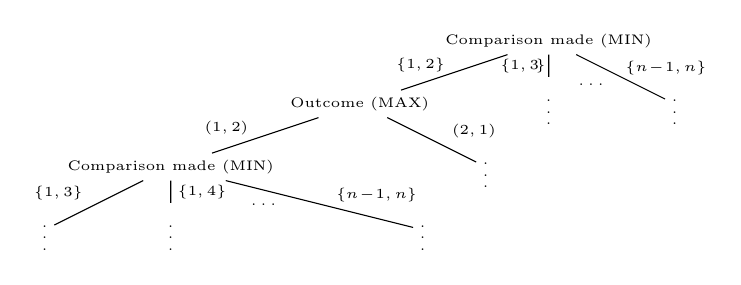
\begin{tikzpicture}[scale=0.8]
  \tiny
  \node (A1) at (0,0) {$\vdots$};
  \node (A2) at (2,0) {$\vdots$};
  \node (A3) at (3.5,0.4) {$\dots$};
  \node (A4) at (6,0) {$\vdots$};

  \node (B1) at (2,1) {Comparison made (MIN)};

  \draw (B1) -- (A1) node[above,pos=0.6, xshift=-0.4cm] {$\{1,3\}$};
  \draw (B1) -- (A2) node[right, midway] {$\{1,4\}$};
  \draw (B1) -- (A4) node[right, pos=0.3, xshift=6mm] {$\{n \!- \! 1,n\}$};

  \node (C1) at (5,2) {Outcome (MAX)};
  \node (B2) at (7,1) {$\vdots$};

  \draw (C1) -- (B2) node[right, pos=0.3, xshift=4mm] {$(2,1)$};

  \draw (B1) -- (C1) node[left, pos=0.7, xshift=-4mm] {$(1,2)$};

  \node (D1) at (8,3) {Comparison made (MIN)};
  \node (C2) at (8,2) {$\vdots$};
  \node (C3) at (8.7,2.3) {$\dots$};
  \node (C4) at (10,2) {$\vdots$};

  \draw (D1) -- (C1) node[left,pos=0.3,xshift=-3mm] {$\{1,2\}$};
  \draw (D1) -- (C2) node[left, midway, xshift=0.5mm] {$\{1,3 \! \}$};
  \draw (D1) -- (C4) node[right, pos=0.3,xshift=2mm] {$\{n \! - \! 1,n\}$};

\end{tikzpicture}
  \caption{Minimax search algorithm}
  \label{fig:minimax_search}
\end{figure}

\subsubsection{Pruning.}
We use the following two pruning criteria to reject posets that are not solvable in the given number of comparisons.

\paragraph{Compatible Solutions.}
The first heuristic uses the number of compatible solutions.
We use the fact, proven in Theorem~\ref{theorem:compatible_log}, that the $\log$ of the number of compatible solutions is a lower bound for the cost of a poset.

\Cref{algo:compatible_solutions} shows an algorithm for computing the number of compatible solutions for a poset.
The algorithm assumes that the elements in the poset are sorted in such a way that an element that is smaller than another has a smaller index.
The calculation of this number first picks a solution element $j$ - since posets are always reduced in the forward search any element is valid - and then counts the number of possible separations into greater and lesser elements, summing up these counts over all solution elements.

\begin{algorithm}[t]
  \centering
  \begin{algorithmic}

    \Function{NumCompatibleSolutions}{$(P, i)$}

    \State{$c \gets 0$}

    \For{$j \in \Omega_P$} \Comment{solutions with $j$ $i$-th smallest}

    \State{$\mathcal{D} \gets \{ \less{P}{j} \setminus \{j\} \}$}% \Comment{downsets containing $\less{P}{j} \setminus \{j\}$}

    \For{$k \in \Omega_P \setminus (\less{P}{j} \cup \greater{P}{j})$}

    \For{$S \in \mathcal{D}$}

    \If{$\less{P}{k} \subseteq S \cup \{ k \}$}
    \State{$\mathcal{D} \gets \mathcal{D} \cup \{ S \cup \{ k \} \}$}
    \EndIf

    \EndFor

    \EndFor

    \State{$c \gets c + |\{S \in \mathcal{D} \mid |S| = i \}|$}

    \EndFor

    \State{\Return{$c$}}

    \EndFunction
\end{algorithmic}

% New Version

% pub fn num_compatible_posets(&self) -> usize {
% debug_assert!(self.is_lower_triangle_matrix());

% let all_less_than = {
%     let mut bitsets = [BitSet::empty(); MAX_N];
%     bitsets
%         .iter_mut()
%         .take(self.n() as usize)
%         .enumerate()
%         .for_each(|(i, bs)| *bs = self.get_all_less_than(i as u8));
%     bitsets
% };

% let mut less_subsets = Vec::with_capacity(1000);

% let mut sum = 0;
% for i in 0..self.n() as usize {
%     // assume the ith element is the solution

%     let less_than_i = all_less_than[i];

%     if less_than_i.len() == self.i() as usize {
%         sum += 1;
%         continue;
%     }
%     if less_than_i.len() > self.i() as usize {
%         continue;
%     }

%     let greater_than_i = self.get_all_greater_than(i as u8);
%     let ordered_with_i = less_than_i.union(greater_than_i);

%     less_subsets.clear();
%     less_subsets.push(less_than_i);

%     for j in 0..self.n() as usize {
%         if j == i || ordered_with_i.contains(j) {
%             continue;
%         }

%         let less_than_j = all_less_than[j];

%         // try adding j to all previous subsets
%         for i in 0..less_subsets.len() {
%             let subset = less_subsets[i];

%             // test if adding j would make a valid subset
%             // we know, that there is no k with p[k] > p[j]
%             if less_than_j.intersect(subset) == less_than_j {
%                 let mut new_subset = subset;
%                 new_subset.insert(j);
%                 less_subsets.push(new_subset);
%             }
%         }
%     }

%     sum += less_subsets
%         .iter()
%         .filter(|s| s.len() == self.i() as usize)
%         .count();
% }

% sum
% }

% Old Version

% pub fn num_compatible_posets(&self) -> usize {
%     let canonified = self.canonify_lower_matrix();

%     let mut sum = 0;
%     for i in 0..canonified.n {
%         // assume the ith element is the solution

%         let less_than_i = canonified.get_all_less_than(i);
%         let greater_than_i = canonified.get_all_greater_than(i);

%         let mut less_subsets = Vec::new();
%         less_subsets.push(BitSet::empty());

%         for j in 0..canonified.n {
%             if j == i || greater_than_i.contains(j as usize) {
%                 continue;
%             }

%             let less_than_j = canonified.get_all_less_than(j);

%             // try adding j to all previous subsets
%             if less_than_i.contains(j as usize) {
%                 // all subsets must contain j to be valid

%                 let mut next_free = 0;
%                 for i in 0..less_subsets.len() {
%                     let subset = less_subsets[i];

%                     // test if adding j would make a valid subset
%                     // we know, that there is no k with p[k] > p[j]
%                     if less_than_j.intersect(subset) == less_than_j {
%                         let mut new_subset = subset;
%                         new_subset.insert(j as usize);
%                         less_subsets[next_free] = new_subset;
%                         next_free += 1;
%                     }
%                 }
%                 less_subsets.truncate(next_free);
%             } else {
%                 for i in 0..less_subsets.len() {
%                     let subset = less_subsets[i];

%                     // test if adding j would make a valid subset
%                     // we know, that there is no k with p[k] > p[j]
%                     if less_than_j.intersect(subset) == less_than_j {
%                         let mut new_subset = subset;
%                         new_subset.insert(j as usize);
%                         less_subsets.push(new_subset);
%                     }
%                 }
%             }
%         }

%         sum += less_subsets
%             .into_iter()
%             .filter(|s| s.len() == canonified.i as usize)
%             .count();
%     }

%     sum
% }
  \caption{An algorithm for computing the number of compatible solutions for a given poset.}
  \label{algo:compatible_solutions}
\end{algorithm}

As an example, the unordered poset $(n,i,\emptyset)$ has $n \cdot \binom{n - 1}{i + 1}$ compatible solutions because for each of the $n$ elements, all separations of the remaining $n - 1$ elements are valid.


\paragraph{Free Comparison.}
The second heuristic attempts to reduce the size of the searched subtree by adding a `useful' comparison to eliminate elements faster.
Explicitly, it searches for unordered elements $u$ and $v$ such that $u$ has as many elements less than it as possible and $v$ as many as possible greater and adds $u < v$ to the poset.
If there is no $u$ with at least two elements less than it or no $v$ with at least $2$ greater, the algorithm aborts the heuristic and resumes regular search.
Otherwise, the new poset is then searched for a solution using the forward search described above without reducing the number of allowed comparisons.
If the new poset is not solvable, we estimate the original is not solvable either.
This heuristic can be slightly improved by maximizing the number of elements smaller than the maximal element and greater than the minimal element.
This is admissible because having a comparison added `for free' does not make the poset harder to solve.

\subsection{Backward Search.} \label{sec:backward}
To develop the backward search, primarily the backward search from~\cite{stober2022lower} was taken as orientation, since it represents a new research area for the selection problem and was not addressed in the previous work by Oksanen~\cite{Oksanen}.

The backward search starts with the set of solved selection problems, and iteratively removes comparisons until the unordered poset is found.
Now, the set of solved problems, even if we restrict ourselves to a fixed cardinality $n$ and rank $i$, will be quite large.
We solve this by only enumerating reduced problems.
With that restriction the starting point of the backward search is $(E_1, 1)$.

\subsubsection{Algorithm.} \label{sec:backward:algorithm}
The input parameters for the backward search are denoted by $n$ and $i$, like in the forward search.
The backward search starts with the solved problem $(E_1, 1)$ and iteratively computes all posets solvable using $k = 1, 2, 3, \dots$ comparisons -- until the unordered poset $(E_n, i)$ is encountered.

Let $A_k$ denote the set of all reduced selection problems solvable using $k$ comparisons.
For all $n$ and $i$, we have $A_0 = \{ (E_1, 1) \}$.

The backward search begins with $A_0$ and iteratively computes, for each problem in $A_k$, the corresponding predecessors, which form the set $A_{k + 1}$.
If $(E_n, i) \in A_l$, then $l$ comparisons are the lower bound to determine the $i$-th smallest element of an $n$-element list.

\subsubsection{Predecessor calculation.} \label{sec:backward:predecessor_calculation}
We begin with a formal definition of a predecessor.

\begin{definition}[Predecessor] \label{definition:predecessor_calculation}
  The problem $(Q, j)$ is a \emph{predecessor} of $(P, i)$ if there is a comparison $(a, b)$, such that
  \begin{enumerate}
    \item $(P, i) = \reduced(\pchild{Q}{a}{b}, j)$ and
    \item $V_j(\pchild{Q}{b}{a}) \le V_i(P)$. % TODO: Why is here `\le`, I think this should be $V_j(\pchild{Q}{b}{a}) + 1 = V_i(P)$
  \end{enumerate}
\end{definition}

Any problem $(Q, j)$ satisfying the first condition of the above definition is called a \emph{potential predecessor}.
In fact the first step to enumerating the predecessors will be to enumerate the potential predecessors.
The second step will be checking the second condition.

\begin{lemma} \label{lemma:predecessor_calculation}
  If $(P, i)$ is solvable in $k$ comparisons and $(Q, j)$ is a predecessor of $(P, i)$, then $(Q, j)$ is solvable in $k + 1$ comparisons.
\end{lemma}

\begin{proof} \label{proof:predecessor_calculation} % todo: update to new def.
  Since $Q$ was not found in any previous round, according to the assumption, it is not solvable in fewer comparisons. % todo: this assumption was never made
  By performing the addition of comparison $(i, j)$ followed by normalization, the poset $P$ is derived, consequently establishing the reachability of $Q$.
  As $P$ is solvable in $k$ comparisons, thus $Q$ is solvable in $k + 1$ comparisons.
  If the comparison is inserted in reverse, according to the assumption, the resulting poset is already in the cache.
  Thus, this path is solvable in at most $k + 1$ comparisons.
\end{proof}

Storing only reduced problems posets is a significant challenge to predecessor enumeration.
Let us illustrate this by looking at a poset $(P, i)$ and its predecessor $(Q, j)$.
We know there is a comparison $(a, b)$ such that $(P, i) = \reduced(\pchild{Q}{a}{b}, j)$.
However it is possible, that the edge $(a, b)$ is not in $P$, because either $a$ or $b$ could have been removed when reducing the problem.
The question is, how can we undo a comparison, that we cannot see?
Then, even if the reduction does not remove $a$ and $b$, there could still be other elements that are removed.
There the challenge is to figure out how many they are and what relations they have.

To address these challenges we will prove two lemmas, the first of which shows that after adding a comparison $(a, b)$ at most one of $\{a, b\}$ will be removed by the reduction.

\begin{lemma} \label{lemma:remove_only_last_element_edge}
  Let $(P, i)$ be a reduced problem.
  Let $(Q, j) = \reduced{(\pchild{P}{a}{b}, i)}$.
  Then, $Q \cap \{a ,b \} \neq \emptyset$.
\end{lemma}

\begin{proof}
  As $(P, i)$ ist reduced, we have $|\less{P}{c}| \le i$ and $|\greater{P}{c}| \le n - i + 1$, where $n = |\Omega_P|$, for every $c \in P$, in particular this also holds for $a$ and $b$.
  Let $P' = \pchild{P}{a}{b}$ and assume $Q \cap \{a ,b \} = \emptyset$.
  Observe that $\less{P'}{a} = \less{P}{a} \le i$ and $\greater{P'}{b} = \greater{P}{b} \le n - i + 1$.
  Thus for $a$ and $b$ to be reduced, we must have $\greater{P'}{a} \ge n - i + 2$ and $\less{P'}{b} \ge i + 1$.
  Note that there are no elements inbetween $a$ and $b$, as they are incomparable in $P$ and there is an Hasse arc between them in $P'$.
  Hence $\greater{P'}{a} \cap \less{P'}{b} = \{a, b\}$, leading to the contradiction $n = |\Omega_{P'}| \ge |\greater{P'}{a} \cup \less{P'}{b}| = |\greater{P'}{a}| + |\less{P'}{b}| - |\greater{P'}{a} \cap \less{P'}{b}| \ge n + 1$.
\end{proof}

The next lemma shows, that the elements removed by the reduction, which are not $a$ or $b$, can be added one after the other.

\begin{lemma}\label{lemma:remove_elements_iteratively}
  Let $(P, i)$ be a reduced problem.
  Let $(Q, j) = \reduced{(\pchild{P}{a}{b}, i)}$.
  Then, $Q \cap \{a, b\} \neq \emptyset$.
  If $(P, i)$ is a predecessor of $(Q, j)$ and $\Omega_P \setminus (\Omega_Q \cup \{a, b\}) \neq \emptyset$, then there is an element $c \in \Omega_P \setminus (\Omega_Q \cup \{a, b\})$ such that $(P|_{\Omega_P \setminus \{c\}}, i')$, where $i' = i - 1$ if $|\greater{\pchild{P}{a}{b}}{c}| \ge n-i+2$ and $i'=i$ otherwise, is a reduced predecessor of $(Q, j)$.
\end{lemma}

\begin{proof}
  Let $R = \Omega_P \setminus (\Omega_Q \cup \{a, b\})$ be the set of elements removed by the reduction.
  It is easy to see that for every $c \in R$ the problem $(P', i')$ where $P' = P|_{\Omega_P \setminus \{c\}}$ and $i' = i - 1$ if $|\greater{\pchild{P}{a}{b}}{c}| \ge n-i+2$ and $i'=i$ otherwise is a predecessor of $(Q, j)$:
  \begin{itemize}
    \item It is obvious that $(Q, j) = \reduced{(\pchild{P'}{a}{b}, i')}$.
    \item $(\pchild{P'}{b}{a}, i')$ is at least as easy solve as $(\pchild{P}{b}{a}, i)$. Thus $V_{i'}(\pchild{P'}{b}{a}) \le V_i(\pchild{P}{b}{a})$.
  \end{itemize}
  The challenge is to find an element $c$, such $P'$ is reduced.
  We define the following sets.
  \begin{align*}
    C^+ & = \{e \in \Omega_P \mid \greater{P}{e} = n - i + 1\}            \\
    C^- & = \{e \in \Omega_P \mid \less{P}{e} = i \}                      \\
    R^+ & = \{c \in V \mid \greater{\pchild{P}{a}{b}}{c} \ge n - i + 2 \} \\
    R^- & = \{c \in V \mid \less{\pchild{P}{a}{b}}{c} \ge i + 1 \}
  \end{align*}
  Note that $R = R^- \cup R^+$.
  The sets $C^-$ and $C^+$ are the critical elements:
  If $P'$ is not reduced, then it is because one of these elements can no longer be the $i$-th smallest.
  To avoid that we need an element $c \in R^+$ that is smaller (in $P$) than all elements in $C^-$.
  By symmetry, any element $c \in R^-$ smaller than all elements in $C^+$ works as well.
  We first show that if we have an element in $R^- \cap C^-$ or $R^+ \cap C^+$, then this property is fulfilled:
  \begin{equation}
    \forall c \in C^+, e \in C^- \colon (c, e) \in P\,\text{.}
  \end{equation}
  Assume we have $c \in C^+, e \in C^-$, but there is no edge $(c, e) \in P$.
  Then the sets $\greater{P}{c}$ and $\less{P}{e}$ are disjoint.
  This is a contradiction as $|\greater{P}{c}| + |\less{P}{e}| = n + 1 > |\Omega_P|$.

  The second step is to show that if $R^- \cap C^- = \emptyset$ and $R^+ \cap C^+ = \emptyset$, then we can pick any $c \in R$.
  We show the following:
  \begin{equation}
    \forall c \in R^-, e \in C^+ \colon (e, c) \in P \text{ or } e \in R^+\,\text{.}
  \end{equation}
  Assume we have $c \in R^-, e \in C^+$.
  By another counting argument we observe that the sets $\less{\pchild{P}{a}{b}}{c}$ and $\greater{P}{e}$ cannot be disjoint:
  Assuming that $\less{\pchild{P}{a}{b}}{c} \cap \greater{P}{e} = \emptyset$ leads to the contradiction $|\less{\pchild{P}{a}{b}}{c}| + |\greater{P}{e}| \ge n + 2$.
  Thus $(e, c) \in \pchild{P}{a}{b}$.
  Hence we have either $(e, c) \in P$ or $(e, a) \in P$.
  If $(e, a) \in P$ but not $(e, c) \in P$, then we have to show $a \neq e$ to obtain $e \in R^+$:
  Assume $a = e$.
  Then $\greater{P}{a} \setminus \{ a \}$ and $\less{\pchild{P}{a}{b}}{c}$ must be disjoint as $(e, c) \notin P$.
  We obtain the contradiction $|\greater{P}{a} \setminus \{ a \}| + |\less{\pchild{P}{a}{b}}{c}| \ge n + 1$.
  By symmetrie we also get
  \begin{equation}
    \forall c \in R^+, e \in C^- \colon (c, e) \in P \text{ or } e \in R^-\,\text{,}
  \end{equation}
  which concludes the proof.
\end{proof}

The computation of a predecessor for a given problem $(P, i)$ comprises three steps:
\begin{enumerate}
  \item Compute predecessors on the same set of elements.
  \item Compute predecessors with exactly one additional element, that is also involved in the comparison.
  \item Starting with the predecessors obtained in the preceding steps add additional elements iteratively.
\end{enumerate}
We describe the individual steps below.\todo{mention only store new predecessors in $A_{k+1}$}

\paragraph{Predecessors on the same set of elements.}
First, we search for all posets with $n_P$ elements that result in poset $P$ after inserting a comparison $a < b$.
In other words, we remove a comparison.
First we compute the potential predecessors.
Each edge in the Hasse diagram of $P$ potentially is a comparison by which $(P, i)$ can be obtained from a predecessor.
A challenge arises from transitive relations, as the insertion of a single comparison can lead to the insertion of multiple transitive relations.
This is illustrated in \Cref{fig:backward_problematic}.
Removing a comparison from (1) can result in either (2) or (3).
Therefore, both (2) and (3) are potential predecessors, even though the same comparison is removed each time.

\begin{figure}[!b]
  \centering
  \begin{tikzpicture}
  \node[circle,draw=black] (A1) at (0, 0) {};
  \node[circle,draw=black] (A2) at (0, 1) {};
  \node[circle,draw=black] (A3) at (0, 2) {};

  \draw (A1) -- (A2) node {};
  \draw (A2) -- (A3) node {};
  \node (AL) at (0, -0.5) {$i = 1$};
  \node (A) at (0, -1) {(1)};


  \node[circle,draw=black] (B1) at (2.5 + 0, 0) {};
  \node[circle,draw=black] (B2) at (2.5 + 0, 2) {};
  \node[circle,draw=black] (B3) at (2.5 + 1, 1) {};

  \draw (B1) -- (B2) node {};
  \node (BL) at (2.5 + 0.5, -0.5) {$i = 1$};
  \node (B) at (2.5 + 0.5, -1) {(2)};


  \node[circle,draw=black] (C1) at (5 + 1, 2) {};
  \node[circle,draw=black] (C2) at (5 + 0, 0) {};
  \node[circle,draw=black] (C3) at (5 + 2, 0) {};

  \draw (C1) -- (C2) node {};
  \draw (C1) -- (C3) node {};
  \node (CL) at (5 + 1, -0.5) {$i = 1$};
  \node (C) at (5 + 1, -1) {(3)};
\end{tikzpicture}
  \caption{Case where further comparisons can be removed transitively by removing a comparison.}
  \label{fig:backward_problematic}
\end{figure}

The second step is to check for each potential predecessor, whether it actually is a predecessor of $(P, i)$.
For a potential predecessor $(Q, j)$ where $(P, i) = \reduced{(\pchild{Q}{a}{b}, j)}$ we do this by checking whether $(\pchild{Q}{a}{b}, j)$ can be solved using at most $V_i(P)$ comparisons.
This is done by checking whether $(\pchild{Q}{a}{b}, j)$ is contained in one of the sets $A_k$ already for $k \le V_i(P)$, which have already been computed at this point.


\paragraph{One additional element, involved in the comparison.}
In the next step, all predecessors with $n + 1$ elements are computed, where the additional element is involved in the comparison.
%    By inserting a comparison followed by canonification, the poset $P$ is obtained such that one element is eliminated during reduction.
%
%    Since the new element is either smaller or larger than the $i$-th smallest element being searched for, the $(i + 1)$-th smallest or the $i$-th smallest element is searched in these predecessors.
%    Given that the poset $P$ is canonified, $i \leq n - 1 - i$ holds for $P$.
%    However, when canonifying a poset with $n + 1$ elements and searching for the $(i + 1)$-th smallest element, it may be necessary to form the dual poset, whereby the $(n + 1) - (i + 1) - 1 = n - i + 1$-th element is searched.
%
We construct the potential predecessor for this case as follows.
We insert a new element into poset $P$ and enumerate all possibilities for the relations between the new element and the existing elements.
We want the predecessor to be reduced, thus it is crucial to ensure that the new element cannot be immediately reduced and that no existing elements can be reduced either.
Since the new element is either smaller or larger than the $i$-th smallest element being searched for, either the $(i + 1)$-th smallest or the $i$-th smallest element is searched in these predecessors.
Furthermore, for each $(Q, j)$ obtained this way, there must exist elements $a$ and $b$ such that $\reduced{(\pchild{Q}{a}{b}, j)} = (P, i)$.
This is required for $(Q, j)$ to be a potential predecessor, and since we additionally want the new element to be part of the comparison, we mandate that either $a$ or $b$ is the new element.
Checking whether the potential predecessors constructed this way are actually predecessors is done the same way as in the preceding step.

For the correctness of our approach note that if we have an arbitrary reduced predecessor, then by removing all elements that are not present in $P$, with the exception of $a$ and $b$ we obtain another reduced predecessor.
We get this by induction on the number of elements removed using \Cref{lemma:remove_elements_iteratively}.
If both $a, b \in P$ then this predecessor is enumerated in the first step.
Otherwise, as proven in \Cref{lemma:remove_only_last_element_edge}, at one of $a, b$ is in $P$ and thus the predecessor is enumerated in this second step.
In the next step we will iteratively enumerate all predecessors by adding additional elements to the ones already found.
That way, we will discover the arbitrary predecessor we started with.

\paragraph{Adding elements iteratively.}
In the third step, new elements are iteratively inserted.
We alternate between generating new potential predecessors and checking which of those are actually predecessors.
We stop when no new predecessors are found or when we reach an upper limit to the number of elements.
New potential predecessors are generated by adding a new element to each predecessor and enumerating all possible relations with the existing elements.
When inserting a new element, it is important to note that it may no longer be the $i$-th smallest but rather the $(i + 1)$-th smallest element being searched, similar to the second step.
We only consider potential predecessors which are reduced and of cause by the addition of the comparison $a < b$ and subsequent reduction, the resulting problem $(P, i)$ should be obtained anew.

\begin{figure}[!b]
  \centering
  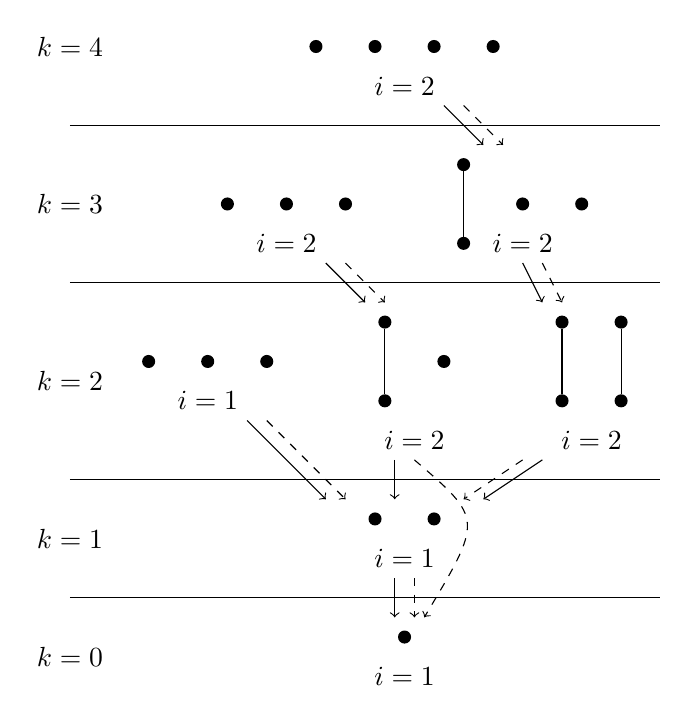
\begin{tikzpicture}

  % Level k = 4
  \node at (-1, 8) {$k=4$};

  \node[circle,fill=black,scale=0.5] (k4_1) at (2.125 + 0 * 0.75, 8) {};
  \node[circle,fill=black,scale=0.5] (k4_2) at (2.125 + 1 * 0.75, 8) {};
  \node[circle,fill=black,scale=0.5] (k4_3) at (2.125 + 2 * 0.75, 8) {};
  \node[circle,fill=black,scale=0.5] (k4_4) at (2.125 + 3 * 0.75, 8) {};
  \node at (2.125 + 0.75 * 1.5, 7.5) {$i=2$};

  \draw[->, dashed] (4, 7.25) -- (4.5, 6.75);
  \draw[->] (3.75, 7.25) -- (4.25, 6.75);

  \draw (-1, 7) -- (6.5, 7);

  % Level k = 3
  \node at (-1, 6) {$k=3$};

  \node[circle,fill=black,scale=0.5] (k3_1) at (1 + 0 * 0.75, 6) {};
  \node[circle,fill=black,scale=0.5] (k3_2) at (1 + 1 * 0.75, 6) {};
  \node[circle,fill=black,scale=0.5] (k3_3) at (1 + 2 * 0.75, 6) {};
  \node at (1 + 0.75, 5.5) {$i=2$};

  \draw[->, dashed] (2.5, 5.25) -- (3, 4.75);
  \draw[->] (2.25, 5.25) -- (2.75, 4.75);

  \node[circle,fill=black,scale=0.5] (k3_4) at (4 + 0 * 0.75, 6.5) {};
  \node[circle,fill=black,scale=0.5] (k3_5) at (4 + 0 * 0.75, 5.5) {};
  \node[circle,fill=black,scale=0.5] (k3_6) at (4 + 1 * 0.75, 6) {};
  \node[circle,fill=black,scale=0.5] (k3_7) at (4 + 2 * 0.75, 6) {};
  \draw (k3_4) -- (k3_5);
  \node at (4 + 0.75, 5.5) {$i=2$};

  \draw[->, dashed] (5, 5.25) -- (5.25, 4.75);
  \draw[->] (4.75, 5.25) -- (5, 4.75);

  \draw (-1, 5) -- (6.5, 5);

  % Level k = 2
  \node at (-1, 3.75) {$k=2$};

  \node[circle,fill=black,scale=0.5] (k2_1) at (0 + 0 * 0.75, 4) {};
  \node[circle,fill=black,scale=0.5] (k2_2) at (0 + 1 * 0.75, 4) {};
  \node[circle,fill=black,scale=0.5] (k2_3) at (0 + 2 * 0.75, 4) {};
  \node at (0 + 0.75, 3.5) {$i=1$};

  \draw[->, dashed] (1.5, 3.25) -- (2.5, 2.25);
  \draw[->] (1.25, 3.25) -- (2.25, 2.25);

  \node[circle,fill=black,scale=0.5] (k2_4) at (3 + 0 * 0.75, 3.5) {};
  \node[circle,fill=black,scale=0.5] (k2_5) at (3 + 0 * 0.75, 4.5) {};
  \node[circle,fill=black,scale=0.5] (k2_6) at (3 + 1 * 0.75, 4) {};
  \draw (k2_4) -- (k2_5);
  \node at (3 + 0.75 * 0.5, 3) {$i=2$};

  \draw[->, dashed] (3.375, 2.75) .. controls (4.25, 2) .. (3.5, 0.75);
  \draw[->] (3.125, 2.75) -- (3.125, 2.25);

  \node[circle,fill=black,scale=0.5] (k2_7) at (5.25 + 0 * 0.75, 3.5) {};
  \node[circle,fill=black,scale=0.5] (k2_8) at (5.25 + 0 * 0.75, 4.5) {};
  \node[circle,fill=black,scale=0.5] (k2_9) at (5.25 + 1 * 0.75, 3.5) {};
  \node[circle,fill=black,scale=0.5] (k2_10) at (5.25 + 1 * 0.75, 4.5) {};
  \draw (k2_7) -- (k2_8);
  \draw (k2_9) -- (k2_10);
  \node at (5.25 + 0.75 * 0.5, 3) {$i=2$};

  \draw[->, dashed] (4.75, 2.75) -- (4, 2.25);
  \draw[->] (5, 2.75) -- (4.25, 2.25);

  \draw (-1, 2.5) -- (6.5, 2.5);

  % Level k = 1
  \node at (-1, 1.75) {$k=1$};

  \node[circle,fill=black,scale=0.5] (k1_1) at (2.875 + 0 * 0.75, 2) {};
  \node[circle,fill=black,scale=0.5] (k1_2) at (2.875 + 1 * 0.75, 2) {};
  \node at (2.875 + 0.75 * 0.5, 1.5) {$i=1$};

  \draw[->, dashed] (3.375, 1.25) -- (3.375, 0.75);
  \draw[->] (3.125, 1.25) -- (3.125, 0.75);

  \draw (-1, 1) -- (6.5, 1);

  % Level k = 0
  \node at (-1, 0.25) {$k=0$};

  \node[circle,fill=black,scale=0.5] (k0_1) at (3.25, 0.5) {};
  \node at (3.25, 0) {$i=1$};
\end{tikzpicture}

  \caption{Search tree for $n = 4$ and $i = 2$.
    Level $k$ contains all posets that can be solved in $k$ comparisons and contribute to the solution for the given parameters $n$ and $i$. \\
    Solid arrows indicate predecessors of a poset, while dashed arrows represent the resulting posets when the reversed comparison is inserted.}
  \label{fig:backward-search-tree}
\end{figure}

\Cref{fig:backward-search-tree} illustrates the posets explored in the backward search for $n = 4$ and $i = 2$.

\subsubsection{Normalform.} \label{sec:backward:normal_form}
Note that the backward search requires a unique normal form and cannot use the approximation used in the forward search.
If our custom canonification fails to produce a unique form, \texttt{nauty} provides the appropriate canonified form.
The following outlines the canonification process:

First, determine whether $i < n - i + 1$ holds.
If not, replace the poset with its dual.
According to \Cref{lemma:dual_poset_allowed}, the solvability of the poset remains unchanged.

Finally, the posets elements are arranged canonically.
The canonic labelling of the elements is provided by \texttt{nauty}.
With this canonical labelling, the poset can be represented canonically.

A potential issue arises if $i = n - i + 1$.
In this case, it is impossible to decide whether $P$ or $P^{-1}$ corresponds to the canonical form based on the value of $i$.

\begin{figure}[!b]
  \centering
  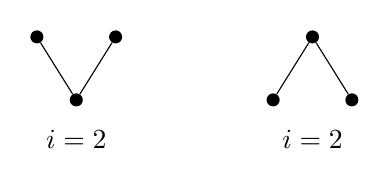
\begin{tikzpicture}
  \node[circle,fill=black,scale=0.5] (A1) at (1, 0) {};
  \node[circle,fill=black,scale=0.5] (A2) at (0.5, 0.8) {};
  \node[circle,fill=black,scale=0.5] (A3) at (1.5, 0.8) {};

  \draw (A1) -- (A2) node {};
  \draw (A1) -- (A3) node {};
  \node (AL) at (1, -0.5) {$i = 2$};


  \node[circle,fill=black,scale=0.5] (B1) at (3 + 1, 0.8) {};
  \node[circle,fill=black,scale=0.5] (B2) at (3 + 0.5, 0) {};
  \node[circle,fill=black,scale=0.5] (B3) at (3 + 1.5, 0) {};

  \draw (B1) -- (B2) node {};
  \draw (B1) -- (B3) node {};
  \node (BL) at (3 + 1, -0.5) {$i = 2$};
\end{tikzpicture}
  \caption{According to \Cref{lemma:dual_poset_allowed}, the two posets are dual to each other.
    In this case, however, \texttt{nauty} cannot be used to transform the posets into each other, since they are two different graphs. This can also be seen in the Hasse diagram, which represents a directed graph, although the arrows are not shown here, but always run implicitly from top to bottom.}
  \label{fig:backward_canonify_problematic}
\end{figure}

% Irgendwo sollte etwas mit Kongruent, nicht Aufgabe von nauty, da dual

In \Cref{fig:backward_canonify_problematic}, the posets as Hasse diagram appear different despite being each other's duals.
To resolve this ambiguity, the dual poset is computed and canonified for each poset where $i = n - i + 1$ holds true.
Subsequently, one of the posets is deterministically selected.
The deterministic selection is realized by comparing the two binary representations.

Since canonification is inevitable for the backward search but consumes significant computational time, all trivial cases are treated manually and only the remaining cases are canonified by \texttt{nauty}.

The manual canonification works as follows:
First, compute the in- and out-degree for each node.
Then assign a hash value to each node based on these degrees, considering the recursive topological structure of adjacent nodes up to a specified depth limit.

Next, sort the nodes according to their hash values.
If all hash values are unique, the graph is in its normal form.
Since it is often the case in the searched posets that two nodes have the same hash values, this case was intercepted.
Let there be $l$ pairs of nodes with identical hash values.
Then there are $2^l$ different possible posets that could correspond to the normal form, since each of the $l$ pairs may or may not be swapped.
Given the realistic assumption that $l$ is small, all $2^l$ permutations can be efficiently iterated.
With the aim of obtaining values for $n = 16$, it follows that there are at most $\frac{n}{2}$ pairs, hence $l \leq 8$ always holds.
All $2^l$ posets are then calculated and one permutation is deterministically selected based on its internal representation, as in the case of the dual poset.
It should be noted that this optimisation only works with pairs of two elements and no longer works if there are three hash values with the same value.

Implementing this canonification preprocessing significantly reduces the number of cases that require \texttt{nauty}, as illustrated in \Cref{table:nauty-ratio}.

\begin{table}[!t]
  \renewcommand{\arraystretch}{1.1}
  \caption{Percentage of canonification requiring \texttt{nauty} for variable $n$ and $i$, where lower values are preferable.}
  \label{table:nauty-ratio}
  \centering
  \small
  \resizebox{\columnwidth}{!}{%
    \begin{tabular}{c|cccccccc}
      $n$ & \multicolumn{8}{c}{$i$}                                                          \\
          & 1                       & 2      & 3     & 4     & 5     & 6     & 7     & 8     \\ \hline
      13  & 0                       & 30.205 & 6.808 & 1.526 & 0.467 & 0.185 & 0.114 &       \\
      14  & 0                       & 33.667 & 7.552 & 1.651 & 0.425 & 0.151 & 0.073 &       \\
      15  & 0                       & 36.390 & 8.184 & 1.678 & 0.459 & 0.132 & 0.065 & 0.041 \\
      16  & 0                       & 39.407 & 8.805 & 1.796 & 0.467 & 0.144 & -     & -     \\
    \end{tabular}%
  }
\end{table}

It is particularly noteworthy that as $i$ increases, the percentage of \texttt{nauty} calls decreases.
For small values of $i$, the high percentage of \texttt{nauty} calls is not critical, as computations for small $i$ are generally quick.

\subsubsection{Optimizations.}

\paragraph{Limit search space.}
As there are potentially many predecessors that cannot contribute to the solution, these are not even calculated.
Many posets can be excluded on the basis of $n$ and $i$.
As illustrated in \Cref{table:n_i_values_calculated}, the search with $n = 7$ and $i = 4$ only considers predecessors that have an `x' in the corresponding row or column.
As the addition of a comparison can reduce $n$ by a maximum of $1$ and therefore $i$ by a maximum of $1$, all other predecessors can be ignored as they can never be used.
For example, no poset with $n = 6$ and $i = 2$ can result in a poset of size $n = 7, i = 4$ by adding a comparison.

The table can be calculated by marking initial $n, i$ with an `x' and then marking recursive the entries for $n - 1, i$ and $n - 1, i - 1$ with an `x', as in each step the new element could be smaller or larger than the $i$-smallest element.

For \Cref{table:n_i_values_calculated}, this means that $n = 6, i = 3$ and $n = 6, i = 4$ should be marked.
It must be noted that $n = 6, i = 4$ does not exist, as the dual poset would be formed at this point.
In this case, only $n = 6, i = 3$ is marked with an `x'.

\begin{table}[!t]
  \renewcommand{\arraystretch}{1.1}
  \caption{Possible predecessors that must be calculated for $n = 7$ and $i = 4$. All predecessors for which the corresponding field is marked with `x' must be calculated.}
  \label{table:n_i_values_calculated}
  \centering
  \small
  \begin{tabular}{c|cccc}
    $n$ & \multicolumn{4}{c}{$i$}             \\
        & 1                       & 2 & 3 & 4 \\ \hline
    7   & -                       & - & - & x \\
    6   & -                       & - & x & - \\
    5   & -                       & x & x & - \\
    4   & x                       & x & - & - \\
    3   & x                       & x & - & - \\
    2   & x                       & - & - & - \\
    1   & x                       & - & - & - \\
  \end{tabular}%
\end{table}

\paragraph{Remaining comparisons.}
In the next step, the minimum number of comparisons that must be removed until the unordered poset is reached is calculated for each predecessor.
This number corresponds to the edges in the corresponding Hasse diagram.
Based on known theoretical upper bounds, all posets containing too many comparisons can be discarded, as they cannot lead to an unordered poset with the remaining comparisons and therefore cannot be considered in the forward search.
Since no more than one comparison can be removed in each step, these posets can be excluded.

\paragraph{Iterative deepening.}
As the theoretical upper bounds are too high in practice, the program uses an iterative deepening approach.
It starts with an upper bound that corresponds to the theoretical lower bound, derived by \Cref{lemma:previous_next_poset} from the smaller values for $n$ and increases this bound iteratively until a solution is finally found.
As it is not possible to save which posets are lost due to the guessed upper bound without considerable effort, the backward search is restarted several times.
Although results from previous rounds are not used, the search space can be considerably reduced and the program can be made more efficient.

\paragraph{Parallelization.} \label{sec:backward:parallelisation}
The backward search can be ideally parallelized by performing the calculation of the predecessors in parallel.
The only two bottlenecks here are read access to the cache and the efficient merging of all partial results.

\begin{table}[!t]
  \renewcommand{\arraystretch}{1.1}
  \caption{Efficiency of parallelism for $n = 13, i = 7$}
  \label{table:backward-parallel}
  \centering
  \small
  \begin{tabular}{l|r|l}
    \textbf{number cores} & \textbf{time} & \textbf{efficiency} \\
    \hline
    $1$                   & 2h 45m        & $1.000$             \\
    $2$                   & 1h 24m        & $0.987$             \\ % this value is super weird, but I ran the test twice -> should be correct
    $3$                   & 1h 1m         & $0.898$             \\
    $6$                   & 31m 46s       & $0.868$             \\
    $12$                  & 17m 4s        & $0.807$             \\
    $24$                  & 9m 9s         & $0.752$             \\
  \end{tabular}
\end{table}

As shown in \Cref{table:backward-parallel} for $n = 13$ and $i = 7$, it can be seen that the backward search scales well with the number of cores.
To set the different times in relation to the number of cores, the efficiency was determined, which represents a direct correlation between the two variables.
This can be calculated as follows
\[
  \text{efficiency} = \cfrac{\text{single-core time}}{\text{number of cores} \cdot \text{multi-core time}}
\]
The higher the efficiency, the better the time scales with the number of cores.

% TODO: subsection?
\begin{figure}[!b]
  \centering
  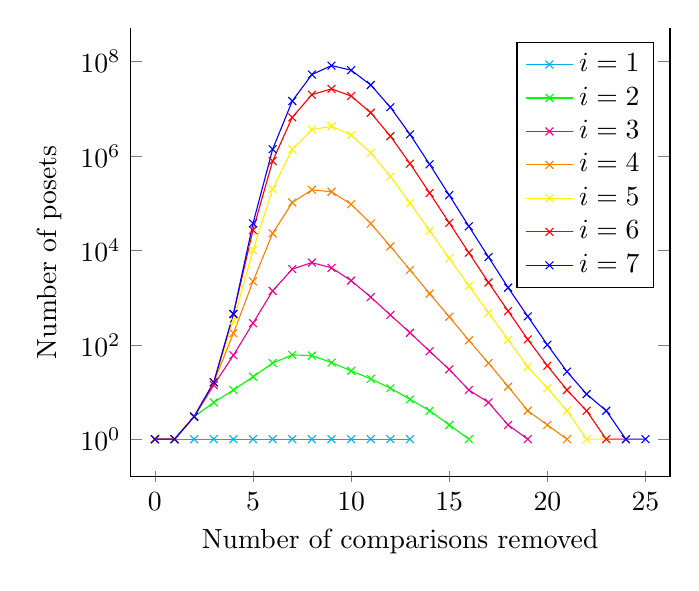
\begin{tikzpicture}
  \begin{axis}[
      ymode=log,
      axis x line = bottom,%x-Achse nur unten
      % x dir=reverse,
      enlarge x limits = .05,%x-Achse erweitern
      x axis line style = {-},%kein Pfeil
      % title = {\dots},
      ylabel={Number of posets},
      xlabel={Number of comparisons removed},
      % only marks,
      cycle list={{mark=x}},
      legend pos=north east,
    ]
    \addlegendentry{$i = 1$}
    \addplot+[cyan] table { %n=14,i=0
        x  y
        0  1
        1  1
        2  1
        3  1
        4  1
        5  1
        6  1
        7  1
        8  1
        9  1
        10 1
        11 1
        12 1
        13 1
      };
    \addlegendentry{$i = 2$}
    \addplot+[green] table { %n=14,i=1
        x y
        0  1
        1  1
        2  3
        3  6
        4  11
        5  21
        6  41
        7  61
        8  59
        9  42
        10 28
        11 19
        12 12
        13 7
        14 4
        15 2
        16 1
      };
    \addlegendentry{$i = 3$}
    \addplot+[magenta] table { %n=14,i=2
        x y
        0  1
        1  1
        2  3
        3  14
        4  60
        5  287
        6  1385
        7  4005
        8  5510
        9  4268
        10 2284
        11 1025
        12 428
        13 180
        14 73
        15 30
        16 11
        17 6
        18 2
        19 1
      };
    \addlegendentry{$i = 4$}
    \addplot+[orange] table { %n=14,i=3
        x y
        0  1
        1  1
        2  3
        3  16
        4  175
        5  2201
        6  22900
        7  103210
        8  191627
        9  174416
        10 94785
        11 37004
        12 12173
        13 3851
        14 1211
        15 392
        16 124
        17 41
        18 13
        19 4
        20 2
        21 1
      };
    \addlegendentry{$i = 5$}
    \addplot+[yellow] table { %n=14,i=4
        x y
        0  1
        1  1
        2  3
        3  16
        4  323
        5  10111
        6  200521
        7  1386176
        8  3607272
        9  4267576
        10 2763862
        11 1162696
        12 367875
        13 100552
        14 26024
        15 6745
        16 1781
        17 474
        18 127
        19 34
        20 12
        21 4
        22 1
        23 1
      };
    \addlegendentry{$i = 6$}
    \addplot+[red] table { %n=14,i=5
        x y
        0  1
        1  1
        2  3
        3  16
        4  446
        5  26921
        6  780123
        7  6588569
        8  19882832
        9  26416869
        10 18631911
        11 8243306
        12 2630332
        13 688904
        14 164372
        15 38334
        16 8918
        17 2084
        18 518
        19 130
        20 36
        21 11
        22 4
        23 1
        24 1
      };
    \addlegendentry{$i = 7$}
    \addplot+[blue] table { % n=14,i=6
        x y
        0  1
        1  1
        2  3
        3  16
        4  452
        5  37236
        6  1389385
        7  14591680
        8  53003482
        9  82198656
        10 65707713
        11 31909980
        12 10770689
        13 2864659
        14 665109
        15 147573
        16 32349
        17 7214
        18 1624
        19 400
        20 100
        21 27
        22 9
        23 4
        24 1
        25 1
      };
  \end{axis}
\end{tikzpicture}
  \caption{Number of posets generated by the backward search for $n = 14$ depending on the number of comparisons for various $i$. Be aware of the logarithmic scale of the y-axis and that the reverse search does not add comparisons, but rather removes them.}
  \label{fig:backward-posets-per-level}
\end{figure}

\Cref{fig:backward-posets-per-level} shows the number of backward search posets for different values of $i$.
It is noticeable that the highest number of posets is searched for all $i$ when there are $8$ to $9$ comparisons left, with a slight tendency towards more comparisons for larger $i$.


\section{Results}

\begin{table}[!t]
  \renewcommand{\arraystretch}{1.1}
  \caption{The minimum number of comparisons needed to select the $i$-th smallest of $n$ elements.
    Values resulting from our work are printed in bold.\todo[inline]{Where to the upper bounds for the ranges come from?}}
  \label{table:num-comparisons}
  \centering
  \small
  \begin{tabular}{c|cccccccc}
    $n$ & \multicolumn{8}{c}{$i$}                                                                                                    \\
        & 1                       & 2  & 3           & 4           & 5           & 6           & 7                & 8                \\ \hline
    1   & 0                                                                                                                          \\
    2   & 1                                                                                                                          \\
    3   & 2                       & 3                                                                                                \\
    4   & 3                       & 4                                                                                                \\
    5   & 4                       & 6  & 6                                                                                           \\
    6   & 5                       & 7  & 8                                                                                           \\
    7   & 6                       & 8  & 10          & 10                                                                            \\
    8   & 7                       & 9  & 11          & 12                                                                            \\
    9   & 8                       & 11 & 12          & 14          & 14                                                              \\
    10  & 9                       & 12 & 14          & 15          & 16                                                              \\
    11  & 10                      & 13 & 15          & 17          & 18          & 18                                                \\
    12  & 11                      & 14 & 17          & 18          & 19          & 20                                                \\
    13  & 12                      & 15 & 18          & 20          & 21          & 22          & 23                                  \\
    14  & 13                      & 16 & 19          & 21          & 23          & 24          & \textbf{25}                         \\
    15  & 14                      & 17 & 20          & 23          & \textbf{24} & \textbf{26} & \textbf{26}      & \textbf{27}      \\
    16  & 15                      & 18 & \textbf{21} & \textbf{24} & \textbf{26} & \textbf{27} & \textbf{28} - 33 & \textbf{28} - 36 \\
  \end{tabular}
\end{table}

The values $V_i(n)$ we calculated as the minimum number of comparisons needed to solve the selection problem for $n \leq 16$ are shown in \Cref{table:num-comparisons}.
We are able to confirm most of the values computed by Oksanen~\cite{Oksanen}.
In particular $V_5(12) = 19$ which is a counter-example to a conjecture of Gasarch~\cite{Gasarch1996} that the optimum can be realized using a ``pair-forming algorithm'', in which the first comparison of any singleton is with another singleton (in this instance, the best pair-forming algorithm requires 20 comparisons).
The values printed in bold have not been known previously.
For $V_7(14)$, $V_6(15)$, $V_7(15)$ and $V_8(15)$ only a range has been known before.
For $V_5(15)$ Oksanen gives a wrong value of $25$ on his website~\cite{Oksanen}.
Curiously enough, running his search algorithm, it produced the correct value $24$.
The values for $n=16$ have not been computed before.
We are able to compute all values for $i \le 6$ and give ranges for $V_7(16)$ and $V_8(16)$.

To verify that the values we calculated are upper bounds, we checked the algorithm certifying each number on each of the $n!$ permutations to ensure it is correct.
Certifying the correctness of the lower bound is near impossible.
We computed every number twice, using two different algorithms, the forward and the backward search.
Thus it is unlikely, that the results are wrong due to a coding error.

\begin{table}[!t]
  \renewcommand{\arraystretch}{1.1}
  \caption{Execution times of different search methods. Times marked with an asterisk gave a non-optimal result \todo[inline]{15, 8 is an old value from the forward search}}
  \label{table:search_algorithms}
  \centering
  \small
  \begin{tabular}{c|c|l|l|l}
    $n$ & $i$ & \textbf{Forward} & \textbf{Backward} & \textbf{Oksanen} \\
    \hline
    12  & 1   & 0.0s             & 0.0s              & 0.0s             \\
    12  & 2   & 0.0s             & 0.2s              & 0.0s             \\
    12  & 3   & 0.4s             & 0.6s              & 0.0s             \\
    12  & 4   & 3.5s             & 0.9s              & 21.4s*           \\
    12  & 5   & 36.1s            & 3.8s              & 4m 59s*          \\
    12  & 6   & 1m 30s           & 18.0s             & 1.9s*            \\
    \hline
    13  & 1   & 0.0s             & 0.0s              & 0.0s             \\
    13  & 2   & 0.0s             & 0.5s              & 0.0s             \\
    13  & 3   & 0.8s             & 1.2s              & 0.2s             \\
    13  & 4   & 13.8s            & 10.3s             & 55.4s            \\
    13  & 5   & 3m 42s           & 44.5s             & 26m 36s          \\
    13  & 6   & 17m 10s          & 3m 22s            & 3h 25m           \\
    13  & 7   & 59m 20s          & 7m 16s            & 16h 10m          \\
    \hline
    14  & 1   & 0.0s             & 0.0s              & 0.0s             \\
    14  & 2   & 0.0s             & 1.3s              & 0.0s             \\
    14  & 3   & 1.4s             & 5.1s              & 0.6s             \\
    14  & 4   & 35.9s            & 33.0s             & 1m 47s           \\
    14  & 5   & 17m 27s          & 7m 1s             & 6h 29m           \\
    14  & 6   & 2h 40m           & 37m 54s           & 4d 10h           \\
    14  & 7   & 14h 40m          & 2h 17m            & >5d              \\
    \hline
    15  & 1   & 0.0s             & 0.0s              & 0.0s             \\
    15  & 2   & 0.1s             & 3.9s              & 0.0s             \\
    15  & 3   & 2.8s             & 24.5s             & 1.4s             \\
    15  & 4   & 2m 24s           & 11m 2s            & 27m 17s          \\
    15  & 5   & 1h 12m           & 22m 11s           & 1d 5h 40m        \\
    15  & 6   & 1d 8h 37m        & 7h 17m            & >5d              \\
    15  & 7   & 4d 23h 37m       & 9h 45m            & >5d              \\
    15  & 8   & 14d 1h 51m       & 1d 3h 7m          & >5d              \\
    \hline
    16  & 1   & 0.0s             & 0.0s              & -                \\
    16  & 2   & 0.2s             & 12.3s             & -                \\
    16  & 3   & 6.4s             & 1m 55.1s          & -                \\
    16  & 4   & 7m 22s           & 52m 9.4s          & -                \\
    16  & 5   & 7h 33m           & 6h 48m 14.8s      & -                \\
    16  & 6   & 6d 11h 21m       & 1d 1h 26m         & -                \\
  \end{tabular}
\end{table}

\Cref{table:search_algorithms} compares the time the different algorithms took to find an optimal selection algorithm.
We ran all algorithms on a machine with two Intel Xeon CPUs, each equipped with $12$ cores ($24$ threads), and a total of $768$ GB of RAM.
The forward search was started with $500$ GB of RAM, and was restarted for each value of $n$ and $i$, so it does not use the cache from previous runs.
The column `Oksanen' shows the times of his program~\cite{Oksanen} on our hardware.
Oksanen's program was started with only $25$ GB because it was designed for only $400$ MB RAM.\todo{why 25Gb?}
The numbers marked with an asterisk indicate that the publicly available version \texttt{1.6} of Oksanen's program did not find an optimal algorithm, even though he has given an optimal algorithm on his website with the unavailable version \texttt{1.1}.
Additionally we measured the number of posets that were stored in the cache after the calculation, which can be seen in \Cref{table:cache_entries}.



\begin{table}[!t]
  \renewcommand{\arraystretch}{1.1}
  \caption{Number of posets stored in the cache after the corresponding search}
  \label{table:cache_entries}
  \centering
  \small
  \begin{tabular}{c|c|r|r}
    $n$ & $i$ & \textbf{Forward Search} & \textbf{Backward Search} \\
    \hline
    13  & 1   & $12$                    & $13$                     \\
    13  & 2   & $329$                   & $245$                    \\
    13  & 3   & $9.7 \cdot 10^3$        & $10.9 \cdot 10^3$        \\
    13  & 4   & $199.7 \cdot 10^3$      & $276.9 \cdot 10^3$       \\
    13  & 5   & $3.7 \cdot 10^6$        & $2.2 \cdot 10^6$         \\
    13  & 6   & $18.1 \cdot 10^6$       & $9.7 \cdot 10^6$         \\
    13  & 7   & $67.6 \cdot 10^6$       & $14.5 \cdot 10^6$        \\
    \hline
    14  & 1   & $13$                    & $14$                     \\
    14  & 2   & $442$                   & $319$                    \\
    14  & 3   & $15.2 \cdot 10^3$       & $19.6 \cdot 10^3$        \\
    14  & 4   & $438.0 \cdot 10^3$      & $644.2 \cdot 10^3$       \\
    14  & 5   & $14.1 \cdot 10^6$       & $13.9 \cdot 10^6$        \\
    14  & 6   & $149.5 \cdot 10^6$      & $84.1 \cdot 10^6$        \\
    14  & 7   & $925.3 \cdot 10^6$      & $263.3 \cdot 10^6$       \\
    \hline
    15  & 1   & $14$                    & $15$                     \\
    15  & 2   & $741$                   & $407$                    \\
    15  & 3   & $23.6 \cdot 10^3$       & $34.9 \cdot 10^3$        \\
    15  & 4   & $1.3 \cdot 10^6$        & $3.1 \cdot 10^6$         \\
    15  & 5   & $53.0 \cdot 10^6$       & $40.0 \cdot 10^6$        \\
    15  & 6   & $1.6 \cdot 10^9$        & $0.73 \cdot 10^9$        \\
    15  & 7   & $5.3 \cdot 10^9$        & $1.3 \cdot 10^9$         \\
    15  & 8   & $15.7 \cdot 10^9$       & $2.2 \cdot 10^9$         \\
    \hline
    16  & 1   & $15$                    & $16$                     \\
    16  & 2   & $990$                   & $520$                    \\
    16  & 3   & $35.8 \cdot 10^3$       & $62.3 \cdot 10^3$        \\
    16  & 4   & $2.4 \cdot 10^6$        & $7.4 \cdot 10^6$         \\
    16  & 5   & $211.1 \cdot 10^6$      & $275.3 \cdot 10^6$       \\
    16  & 6   & $3.6 \cdot 10^9$        & $2.6 \cdot 10^9$         \\
  \end{tabular}
\end{table}


\section{Conclusion and Open Questions}

%Using computer search based on the work of Oksanen we were able to write our own version of a search program for selecting the $i$-th element of a list of $n$ elements (see: \href{https://github.com/JGDoerrer/selection_generator}{Github}) and not only confirming the found solutions of Oksanen for the problem but also improving some entries (e.g. $n = 15, i = 5$).
%Further we added some more numbers and therefore algorithms to \Cref{table:num-comparisons} for higher $n$ and $i$.

As stated in the motivation before: the road is better than the inn.
Along the way we improved the forward search using a heuristic based on compatible solutions and evaluated a new algorithmic approach -- the backward search coming to a final conclusion that both are valid.
%If you want to use the program to generate more optimal numbers and therefore algorithms one should have quite some time and good hardware in form of a high CPU count and as much RAM as possible (see: \Cref{sec:hardware} for our used hardware).
%Right now one should use the backward search due to the lower RAM footprint and scaling with the CPU count.
%
%The latest version of our software can be found on github (\url{https://github.com/JGDoerrer/selection_generator}).
Between the structural constraints of our algorithms and the available hardware, $n=16$ is likely the limit of feasible calculation for the current state.
%but with speedup in orders of magnitude even towards the end of development 
We believe that higher $n$ are realistic with new algorithmic ideas and conclude this work by talking about promising directions for further research.

\paragraph{Bidirectional Search.}
The classical meet in the middle approach for a bidirectional search will not work for the selection problem.
This is illustrated in \Cref{fig:backward_forward_count_13_6}:
assume the two searches meet at the point where $11$ comparisons have been performed and $12$ remain.
When reaching the meeting point the forward search has explored $99.006\%$ of its search space and the backward has explored $99.349\%$ of its search space.
%Thus at the meeting point both searches have already explored most of their search space.

\begin{figure}[!b]
  \centering
  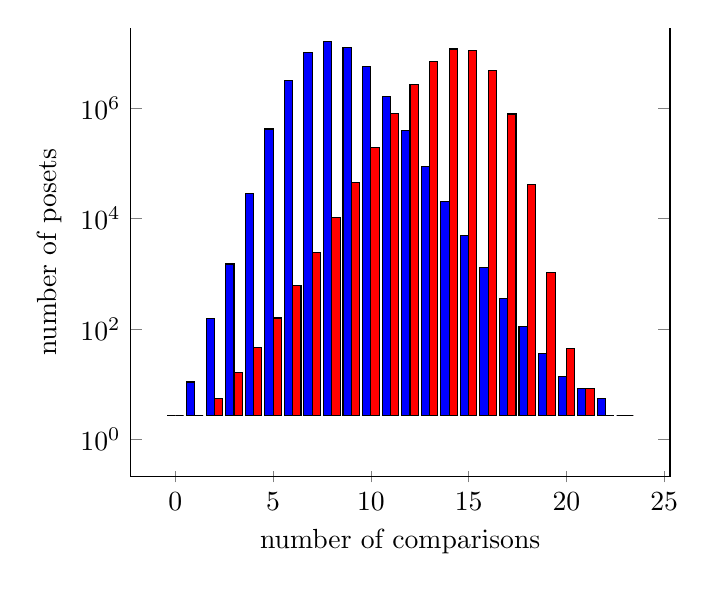
\begin{tikzpicture}
  \begin{axis}[
      ybar,
      ymode=log,
      axis x line = bottom,%x-Achse nur unten
      enlarge x limits = .1,%x-Achse erweitern
      x axis line style = {-},%kein Pfeil
      bar width=3pt,
      ylabel={number of posets},
      xlabel={number of comparisons},
      % legend cell align=left,
      % legend pos=outer north east,
      % legend style={at={(0.5,-0.2)},anchor=north}, % draw=none
    ]
    % \addlegendentry{forward search}
    \addplot[fill=blue,shift={(1pt, 0)}] table {
        x y
        0  1
        1  4
        2  57
        3  552
        4  10397
        5  154828
        6  1166640
        7  3770182
        8  5941732
        9  4726819
        10 2096404
        11 604582
        12 143058
        13 32460
        14 7450
        15 1823
        16 471
        17 132
        18 41
        19 13
        20 5
        21 3
        22 2
        23 1
      };
    % \addlegendentry{backward search}
    \addplot[fill=red,shift={(-1pt, 0)}] table {
        x y
        23 1
        22 1
        21 3
        20 16
        19 381
        18 15227
        17 290138
        16 1750707
        15 4058631
        14 4368185
        13 2592437
        12 1006071
        11 291970
        10 72346
        9  16728
        8  3898
        7  893
        6  227
        5  58
        4  17
        3  6
        2  2
        1  1
        0  1
      };
  \end{axis}
\end{tikzpicture}

Treff: 11
  \caption{Number of posets depending on the number of comparisons for $n = 13$ and $i = 7$ (red: backward search, blue: forward search).}
  \label{fig:backward_forward_count_13_6}
\end{figure}

An alternative approach to the bidirectional search would be to first run the backward search, but restrict it to problems with specific properties.
E.g.\ enumerate only those problems $(P, i)$ in $A_k$ with $\mathcal{C}(P, i) \ge \alpha \cdot 2^k$ for some $\alpha \in [0, 1]$.
Then the subsequent forward search can look up problems with a large number of compatible solutions, which are presumably hard to solve, in the results of the backward search, and only has to explore problems with a small number of linear extensions, which we estimate to be easier to solve.

The number of compatible solutions might not be the best metric to separate backward and forward search.
We observed that the number of comparisons required to solve a selection problem is typically about twice the lower bound obtained from the number of compatible solutions.
This makes sense, as lower bound it gives for the median is $n + \smallO(n)$, which is far from the best known asymptotic lower bound $2n + \smallO(n)$.

\paragraph{Improved Weight Function.}
A better lower bound can be obtained if instead of just counting the compatible solutions we assign a weight to each solution.
It is relatively easy to create a weight function that leads to a lower bound of $1.5n + \smallO(n)$ for the median.
We also tried to create a weight function, that mimics the techniques used to obtain the $2n + \smallO(n)$ bound in~\cite{bent1985finding}.
However, that lead to a negative $4\sqrt{n}$ term in the resulting lower bound, for $n \le 16$ cancelling out any improvement over just counting the compatible solutions.

\paragraph{Yao's conjecture.}
Yao conjectured that finding the $i$-th smallest of $n$ elements is at least as hard as finding an $n$-element subset $S$ of $m$ elements, where $m > n$, and an element $s \in S$ such that $s$ ist the $i$-th smallest element in $S$~\cite{yao1974lower}.
It is unclear, whether her conjecture holds.
If true, this conjecture would imply a $2.5n + \smallO(n)$ algorithm for computing the median.
By adapting the search algorithm we presented, one could search for counter examples to the conjecture.



\section*{Acknowledgments}
\todo[inline]{tbd}

\bibliography{biblio}


\clearpage
\appendix


\section{Example.}
\begin{figure}[!b]
  \centering
  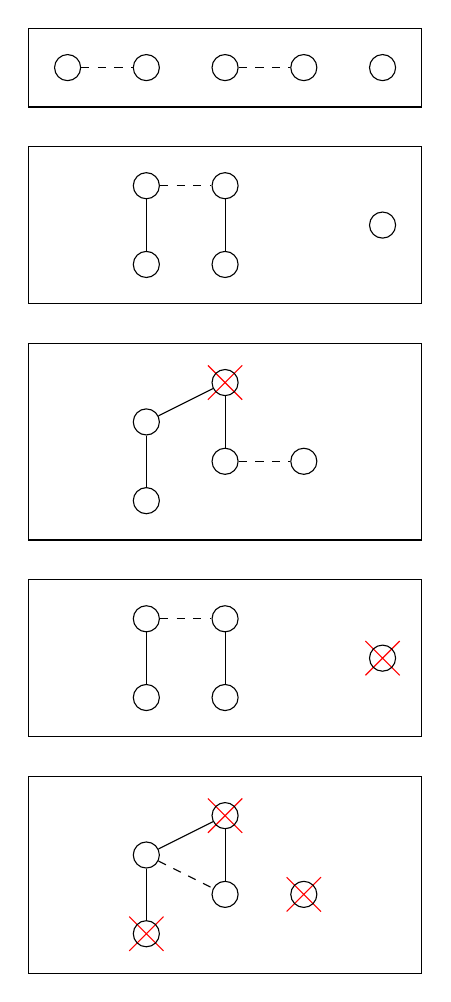
\begin{tikzpicture}[tcancel/.append style={draw=#1, cross out, inner sep=6pt}]
  \draw(-.5, -.5) rectangle (4.5, .5);
  \node[circle,draw=black] (A1) at (0, 0) {};
  \node[circle,draw=black] (A2) at (1, 0) {};
  \node[circle,draw=black] (A3) at (2, 0) {};
  \node[circle,draw=black] (A4) at (3, 0) {};
  \node[circle,draw=black] (A5) at (4, 0) {};

  \draw[dashed] (A1) -- (A2) node {};
  \draw[dashed] (A3) -- (A4) node {};

  \draw(-0.5, -3.0) rectangle (4.5, -1.0);
  \node[circle,draw=black] (B1) at (1.0, 0 - 2.5) {};
  \node[circle,draw=black] (B2) at (1.0, 1 - 2.5) {};
  \node[circle,draw=black] (B3) at (2.0, 0 - 2.5) {};
  \node[circle,draw=black] (B4) at (2.0, 1 - 2.5) {};
  \node[circle,draw=black] (B5) at (4.0, 0.5 - 2.5) {};

  \draw (B1) -- (B2) node {};
  \draw (B3) -- (B4) node {};
  \draw[dashed] (B2) -- (B4) node {};

  \draw(-0.5, -6.0) rectangle (4.5, -3.5);
  \node[circle,draw=black] (C1) at (1, 0 - 5.5) {};
  \node[circle,draw=black] (C2) at (1, 1 - 5.5) {};
  \node[circle,draw=black,tcancel=red] (C3) at (2, 1.5 - 5.5) {};
  \node[circle,draw=black] (C3) at (2, 1.5 - 5.5) {};
  \node[circle,draw=black] (C4) at (2, .5 - 5.5) {};
  \node[circle,draw=black] (C5) at (3, .5 - 5.5) {};

  \draw (C1) -- (C2) node {};
  \draw (C3) -- (C4) node {};
  \draw (C2) -- (C3) node {};
  \draw[dashed] (C4) -- (C5) node {};

  \draw(-0.5, -8.5) rectangle (4.5, -6.5);
  \node[circle,draw=black] (D1) at (1.0, 0 - 8) {};
  \node[circle,draw=black] (D2) at (1.0, 1 - 8) {};
  \node[circle,draw=black] (D3) at (2.0, 0 - 8) {};
  \node[circle,draw=black] (D4) at (2.0, 1 - 8) {};
  \node[circle,draw=black,tcancel=red] (D5) at (4.0, 0.5 - 8) {};
  \node[circle,draw=black] (D5) at (4.0, 0.5 - 8) {};

  \draw (D1) -- (D2) node {};
  \draw (D3) -- (D4) node {};
  \draw[dashed] (D2) -- (D4) node {};

  \draw(-0.5, -11.5) rectangle (4.5, -9.);
  \node[circle,draw=black,tcancel=red] (E1) at (1, 0 - 11.0) {};
  \node[circle,draw=black] (E1) at (1, 0 - 11.0) {};
  \node[circle,draw=black] (E2) at (1, 1 - 11.0) {};
  \node[circle,draw=black,tcancel=red] (E3) at (2, 1.5 - 11.0) {};
  \node[circle,draw=black] (E3) at (2, 1.5 - 11.0) {};
  \node[circle,draw=black] (E4) at (2, .5 - 11.0) {};
  \node[circle,draw=black,tcancel=red] (E5) at (3, .5 - 11.0) {};
  \node[circle,draw=black] (E5) at (3, .5 - 11.0) {};

  \draw (E1) -- (E2) node {};
  \draw (E3) -- (E4) node {};
  \draw (E2) -- (E3) node {};
  \draw[dashed] (E2) -- (E4) node {};
\end{tikzpicture}
  \caption{Finding the median $i = 3$ of $n = 5$ values using six comparisons.\todo[inline]{Can we make this smaller/ same style as the other figures?}}
  \label{fig:median_of_5}
\end{figure}
A good visual example is finding the median $i = 3$ in a list of $n = 5$ elements.
\Cref{fig:median_of_5} illustrate the search of the median using Hasse diagrams.
Each step shows the comparisons to be performed next as a dashed line.
A Hasse diagram of the order of relation found so far (smaller=lower, larger=higher) is shown as the solid lines.
The red crosses indicate elements that have been found to be greater or smaller than three other elements and therefore are disqualified for the median.
The larger element of the final comparison is the median.
This is also the optimal algorithm for $i = 3$ and $n = 5$.


\todo[inline]{Details on how potential predecessors are computed (especially regarding transitive relations).}

\todo[inline]{Approximate normal form for forward search.}



\section{Used Soft- and Hardware.} \label{sec:hardware}

Our results were facilitated by advancements in both hardware and software.
All versions of the software used are listed in the \Cref{table:command_outputs}.
For hardware, we employed two Intel Xeon E5-2650v4 CPUs (2.20\,GHz, 12 Cores/24 Threads, 30\,MB L3-Cache per CPU), and a total of $768$ GB of RAM.

\begin{table}[!t]
  \renewcommand{\arraystretch}{1.1}
  \caption{Specific versions on the software used.}
  \label{table:command_outputs}
  \centering
  \small
  \begin{tabular}{l|l}
    \textbf{Command}  & \textbf{Output}                   \\ \hline
    \texttt{rustc -V} & rustc 1.77.2                      \\ \hline
    \texttt{clang -v} & Ubuntu clang version 14.0.0-1     \\ \hline
    \texttt{uname -a} & Linux plankton 5.15.0-105-generic \\
  \end{tabular}
\end{table}

\end{document}
